% Drawing 144/07-11 -- folder 144, batch 07, archive page 139 (PDF page 140).
% Transcription: reprise au propre du diagramme IV de la p.~137, en trois blocs de cubes. Ligne supérieure : $N^?_{0\rho}$ (biffé) $\overset{2}{\hookrightarrow} N^?_\rho$ ; $N^?_\rho$ (biffé) ; $N^?_\rho \hookrightarrow \mathcal{M}^? \overset{6}{\hookrightarrow} \mathcal{M}$ ; $\mathcal{M}^?_0\overset{2}{\hookrightarrow}\mathcal{M}^!$. Ligne médiane : $Z^!_{0\rho} = \mathcal{M}(\bar{\jmath})\overset{2}{\hookrightarrow}Z^!_\rho\hookrightarrow\mathcal{M}'^!\overset{6}{\hookrightarrow}\mathcal{M}'$ ; $\mu_{\tau'}\overset{2}{\hookrightarrow}D_{\tau'}\hookrightarrow\Pi_{\tau'}\overset{6}{\hookrightarrow}\mathfrak{S}$ ; $\mathcal{M}'^!_0\hookrightarrow\mathcal{M}'^!$ ; $1\overset{2}{\hookrightarrow}\underline\mu\hookrightarrow\underline\Pi\overset{6}{\hookrightarrow}\underline{\mathfrak{S}}^+$. Ligne inférieure : $\underline\Pi_0\overset{2}{\hookrightarrow}\underline\Pi$, $\mathcal{M}'$ ; puis $\underline{\mathfrak{S}}^+$ au bas d'une arête d'indice 6. Arêtes verticales et diagonales d'indice 2 ; deux arcs pointillés relient $\underline\Pi$ et $\underline{\mathfrak{S}}^+$ (bloc de droite) à $\underline\Pi$ et $\underline{\mathfrak{S}}^+$ (bloc de gauche). Au crayon, en bas de page, une esquisse antérieure du même diagramme : $N^?_{0\rho}$ (biffé), $N^?_\rho$, $N_\rho$, $\mathcal{M}$ ; $Z^!_{0\rho} = \mathcal{M}(\bar{\jmath})$, $Z^!_\rho$, $Z_\rho$, $\mathcal{M}'$ ; $\mu_{\tau'}$, $D_{\tau'}$, $D_\rho$, $\mathfrak{S}$ ; $\mathcal{M}'^!_0$, $\mathcal{M}'^!$ ; $\underline\mu$, $L_\rho$, $\underline{\mathfrak{S}}^+$ ; $\underline\Pi_0$, $\underline\Pi$.
% Kind: fair copy of diagram IV in three blocks of cubes, with an earlier pencil sketch. Method 2 (schematic redraw from the facsimile). Status: partial.
% Notes: Top: the inked fair copy (three blocks of cubes): N^?_{0 rho} (struck, grey) -2-> N^?_rho; N^?_rho -> M^? -6-> M; M^?_0 -2-> M^!; Z^!_{0 rho} = M(j bar) -2-> Z^!_rho -> M'^! -6-> M'; mu_tau' -2-> D_tau' -> Pi_tau' -6-> S; M'^!_0 -> M'^!; 1 -2-> mu -> Pi -6-> S^+; Pi_0 -2-> Pi, M', and S^+ at the foot of an edge of index 6; the two dashed arcs join Pi and S^+ of the right block to those of the left block. Bottom: the earlier pencil sketch of the same diagram (read on a contrast-enhanced crop), all in pencil; its strokes are a reading. Arrow directions of the vertical and diagonal edges, and which strokes are hooks, are a reading throughout; the small dashed arcs between the N^? at the top are drawn as plain strokes.
% Coordinates: 1 unit = 1 mm = 1/100 of the crop width (bbox in page fractions: [0.15, 0.07, 0.85, 0.86]).
% Redrawn by Claude (claude-opus-5-5), issue #73, 2026-11-07; not checked by a human; not compiled (no TeX in the session).
% Rights: reproduces part of the work -- behind RENDER_TRANSCRIPTS, never published by itself.
\documentclass[tikz,border=3pt]{standalone}
\usepackage{amsmath,amssymb}
\usetikzlibrary{patterns,arrows.meta}
\tikzset{pencil/.style={black!45}, struck/.style={black!35}, mark/.style={circle,draw,inner sep=1.3pt}, pt/.style={circle,fill,inner sep=0.9pt}, opt/.style={circle,draw,fill=white,inner sep=1.1pt}}
\begin{document}
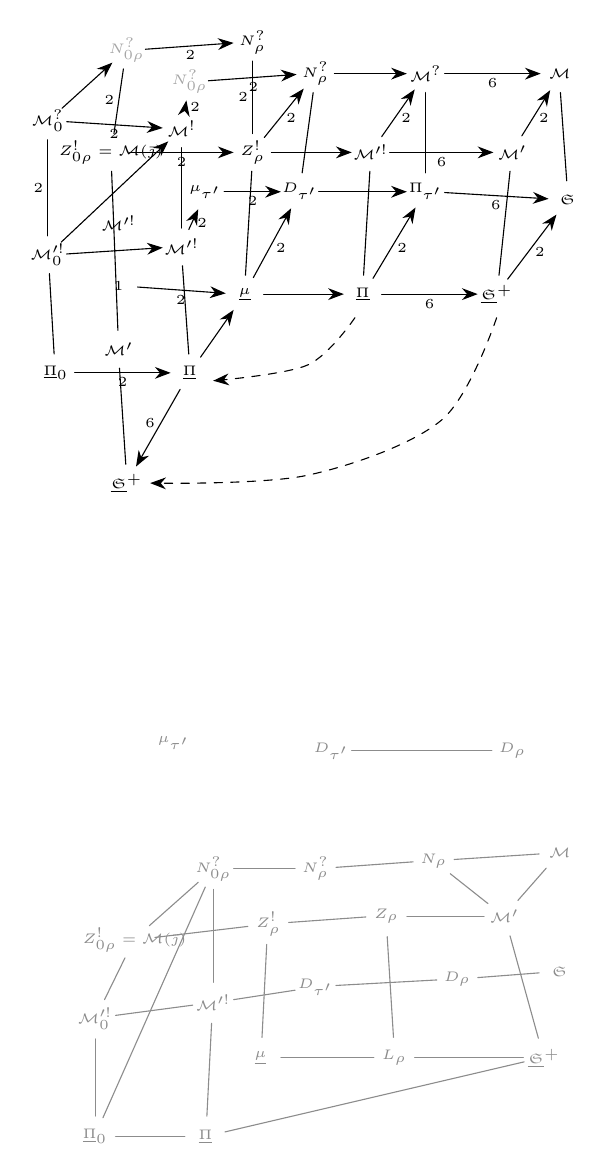
\begin{tikzpicture}[x=1mm,y=1mm,line cap=round,line join=round,font=\scriptsize]
\node[inner sep=1pt,struck] at (22,-15) {\tiny $N^?_{0\rho}$};
\node[inner sep=1pt] at (38,-14) {\tiny $N^?_\rho$};
\node[inner sep=1pt,struck] at (30,-19) {\tiny $N^?_{0\rho}$};
\node[inner sep=1pt] at (46,-18) {\tiny $N^?_\rho$};
\node[inner sep=1pt] at (60,-18) {\tiny $\mathcal M^?$};
\node[inner sep=1pt] at (77,-18) {\tiny $\mathcal M$};
\node[inner sep=1pt] at (12,-24) {\tiny $\mathcal M^?_0$};
\node[inner sep=1pt] at (29,-25) {\tiny $\mathcal M^!$};
\node[inner sep=1pt] at (20,-28) {\tiny $Z^!_{0\rho}=\mathcal M(\bar\jmath)$};
\node[inner sep=1pt] at (38,-28) {\tiny $Z^!_\rho$};
\node[inner sep=1pt] at (53,-28) {\tiny $\mathcal M'^!$};
\node[inner sep=1pt] at (71,-28) {\tiny $\mathcal M'$};
\node[inner sep=1pt] at (21,-37) {\tiny $\mathcal M'^!$};
\node[inner sep=1pt] at (32,-33) {\tiny $\mu_{\tau'}$};
\node[inner sep=1pt] at (44,-33) {\tiny $D_{\tau'}$};
\node[inner sep=1pt] at (60,-33) {\tiny $\Pi_{\tau'}$};
\node[inner sep=1pt] at (78,-34) {\tiny $\mathfrak S$};
\node[inner sep=1pt] at (12,-41) {\tiny $\mathcal M'^!_0$};
\node[inner sep=1pt] at (29,-40) {\tiny $\mathcal M'^!$};
\node[inner sep=1pt] at (21,-45) {\tiny $1$};
\node[inner sep=1pt] at (37,-46) {\tiny $\underline\mu$};
\node[inner sep=1pt] at (52,-46) {\tiny $\underline\Pi$};
\node[inner sep=1pt] at (69,-46) {\tiny $\underline{\mathfrak S}^+$};
\node[inner sep=1pt] at (13,-56) {\tiny $\underline\Pi_0$};
\node[inner sep=1pt] at (30,-56) {\tiny $\underline\Pi$};
\node[inner sep=1pt] at (21,-53) {\tiny $\mathcal M'$};
\node[inner sep=1pt] at (22,-70) {\tiny $\underline{\mathfrak S}^+$};
\draw[-{Stealth[length=2mm]}] (24.4,-14.9) -- (35.6,-14.1);
\node[inner sep=1pt] at (30.1,-15.7) {\tiny $2$};
\draw[-{Stealth[length=2mm]}] (32.4,-18.9) -- (43.6,-18.1);
\node[inner sep=1pt] at (38.1,-19.7) {\tiny $2$};
\draw[-{Stealth[length=2mm]}] (48.4,-18) -- (57.6,-18);
\draw[-{Stealth[length=2mm]}] (62.4,-18) -- (74.6,-18);
\node[inner sep=1pt] at (68.5,-19.2) {\tiny $6$};
\draw[-{Stealth[length=2mm]}] (14.4,-24.1) -- (26.6,-24.9);
\node[inner sep=1pt] at (20.4,-25.7) {\tiny $2$};
\draw[-{Stealth[length=2mm]}] (22.4,-28) -- (35.6,-28);
\node[inner sep=1pt] at (29,-29.2) {\tiny $2$};
\draw[-{Stealth[length=2mm]}] (40.4,-28) -- (50.6,-28);
\draw[-{Stealth[length=2mm]}] (55.4,-28) -- (68.6,-28);
\node[inner sep=1pt] at (62,-29.2) {\tiny $6$};
\draw[-{Stealth[length=2mm]}] (34.4,-33) -- (41.6,-33);
\node[inner sep=1pt] at (38,-34.2) {\tiny $2$};
\draw[-{Stealth[length=2mm]}] (46.4,-33) -- (57.6,-33);
\draw[-{Stealth[length=2mm]}] (62.4,-33.1) -- (75.6,-33.9);
\node[inner sep=1pt] at (68.9,-34.7) {\tiny $6$};
\draw[-{Stealth[length=2mm]}] (14.4,-40.9) -- (26.6,-40.1);
\draw[-{Stealth[length=2mm]}] (23.4,-45.1) -- (34.6,-45.9);
\node[inner sep=1pt] at (28.9,-46.7) {\tiny $2$};
\draw[-{Stealth[length=2mm]}] (39.4,-46) -- (49.6,-46);
\draw[-{Stealth[length=2mm]}] (54.4,-46) -- (66.6,-46);
\node[inner sep=1pt] at (60.5,-47.2) {\tiny $6$};
\draw[-{Stealth[length=2mm]}] (15.4,-56) -- (27.6,-56);
\node[inner sep=1pt] at (21.5,-57.2) {\tiny $2$};
\draw (21.6,-17.4) -- (20.4,-25.6);
\node[inner sep=1pt] at (19.8,-21.3) {\tiny $2$};
\draw (38,-16.4) -- (38,-25.6);
\node[inner sep=1pt] at (36.8,-21) {\tiny $2$};
\draw (45.7,-20.4) -- (44.3,-30.6);
\draw (60,-20.4) -- (60,-30.6);
\draw (77.1,-20.4) -- (77.9,-31.6);
\draw (12,-26.4) -- (12,-38.6);
\node[inner sep=1pt] at (10.8,-32.5) {\tiny $2$};
\draw (29,-27.4) -- (29,-37.6);
\draw (37.9,-30.4) -- (37.1,-43.6);
\draw (52.9,-30.4) -- (52.1,-43.6);
\draw (70.7,-30.4) -- (69.3,-43.6);
\draw (12.2,-43.4) -- (12.8,-53.6);
\draw (29.1,-42.4) -- (29.9,-53.6);
\draw (21.1,-55.4) -- (21.9,-67.6);
\draw (20.1,-30.4) -- (20.9,-50.6);
\draw[-{Stealth[length=2mm]}] (13.8,-22.4) -- (20.2,-16.6);
\draw[-{Stealth[length=2mm]}] (29.4,-22.6) -- (29.6,-21.4);
\node[inner sep=1pt] at (30.7,-22.2) {\tiny $2$};
\draw[-{Stealth[length=2mm]}] (39.5,-26.1) -- (44.5,-19.9);
\node[inner sep=1pt] at (42.9,-23.7) {\tiny $2$};
\draw[-{Stealth[length=2mm]}] (54.4,-26) -- (58.6,-20);
\node[inner sep=1pt] at (57.5,-23.7) {\tiny $2$};
\draw[-{Stealth[length=2mm]}] (72.2,-25.9) -- (75.8,-20.1);
\node[inner sep=1pt] at (75,-23.6) {\tiny $2$};
\draw[-{Stealth[length=2mm]}] (29.9,-37.8) -- (31.1,-35.2);
\node[inner sep=1pt] at (31.6,-37) {\tiny $2$};
\draw[-{Stealth[length=2mm]}] (38.1,-43.9) -- (42.9,-35.1);
\node[inner sep=1pt] at (41.6,-40.1) {\tiny $2$};
\draw[-{Stealth[length=2mm]}] (53.3,-44) -- (58.7,-35);
\node[inner sep=1pt] at (57,-40.1) {\tiny $2$};
\draw[-{Stealth[length=2mm]}] (70.4,-44.1) -- (76.6,-35.9);
\node[inner sep=1pt] at (74.5,-40.7) {\tiny $2$};
\draw[-{Stealth[length=2mm]}] (13.7,-39.4) -- (27.3,-26.6);
\draw[-{Stealth[length=2mm]}] (31.4,-54) -- (35.6,-48);
\draw[-{Stealth[length=2mm]}] (28.8,-58.1) -- (23.2,-67.9);
\node[inner sep=1pt] at (25,-62.4) {\tiny $6$};
\draw[dashed,-{Stealth[length=2mm]}] plot[smooth, tension=0.55] coordinates {(51,-49) (45,-55) (33,-57)};
\draw[dashed,-{Stealth[length=2mm]}] plot[smooth, tension=0.55] coordinates {(69,-49) (62,-62) (45,-69) (25,-70)};
\node[inner sep=1pt,pencil] at (33,-119) {\tiny $N^?_{0\rho}$};
\node[inner sep=1pt,pencil] at (46,-119) {\tiny $N^?_\rho$};
\node[inner sep=1pt,pencil] at (61,-118) {\tiny $N_\rho$};
\node[inner sep=1pt,pencil] at (77,-117) {\tiny $\mathcal M$};
\node[inner sep=1pt,pencil] at (23,-128) {\tiny $Z^!_{0\rho}=\mathcal M(\bar\jmath)$};
\node[inner sep=1pt,pencil] at (40,-126) {\tiny $Z^!_\rho$};
\node[inner sep=1pt,pencil] at (55,-125) {\tiny $Z_\rho$};
\node[inner sep=1pt,pencil] at (70,-125) {\tiny $\mathcal M'$};
\node[inner sep=1pt,pencil] at (18,-138) {\tiny $\mathcal M'^!_0$};
\node[inner sep=1pt,pencil] at (33,-136) {\tiny $\mathcal M'^!$};
\node[inner sep=1pt,pencil] at (46,-134) {\tiny $D_{\tau'}$};
\node[inner sep=1pt,pencil] at (64,-133) {\tiny $D_\rho$};
\node[inner sep=1pt,pencil] at (77,-132) {\tiny $\mathfrak S$};
\node[inner sep=1pt,pencil] at (39,-143) {\tiny $\underline\mu$};
\node[inner sep=1pt,pencil] at (56,-143) {\tiny $L_\rho$};
\node[inner sep=1pt,pencil] at (75,-143) {\tiny $\underline{\mathfrak S}^+$};
\node[inner sep=1pt,pencil] at (18,-153) {\tiny $\underline\Pi_0$};
\node[inner sep=1pt,pencil] at (32,-153) {\tiny $\underline\Pi$};
\node[inner sep=1pt,pencil] at (28,-103) {\tiny $\mu_{\tau'}$};
\node[inner sep=1pt,pencil] at (48,-104) {\tiny $D_{\tau'}$};
\node[inner sep=1pt,pencil] at (71,-104) {\tiny $D_\rho$};
\draw[pencil] (35.6,-119) -- (43.4,-119);
\draw[pencil] (48.6,-118.8) -- (58.4,-118.1);
\draw[pencil] (63.6,-117.8) -- (74.4,-117.1);
\draw[pencil] (25.6,-127.7) -- (37.4,-126.3);
\draw[pencil] (42.6,-125.8) -- (52.4,-125.1);
\draw[pencil] (57.6,-125) -- (67.4,-125);
\draw[pencil] (20.6,-137.6) -- (30.4,-136.3);
\draw[pencil] (35.6,-135.6) -- (43.4,-134.4);
\draw[pencil] (48.6,-133.8) -- (61.4,-133.1);
\draw[pencil] (66.6,-132.8) -- (74.4,-132.2);
\draw[pencil] (41.6,-143) -- (53.4,-143);
\draw[pencil] (58.6,-143) -- (72.4,-143);
\draw[pencil] (20.6,-153) -- (29.4,-153);
\draw[pencil] (34.5,-152.4) -- (72.5,-143.5);
\draw[pencil] (50.6,-104) -- (68.4,-104);
\draw[pencil] (33,-121.6) -- (33,-133.4);
\draw[pencil] (18,-140.6) -- (18,-150.4);
\draw[pencil] (32.8,-138.6) -- (32.2,-150.4);
\draw[pencil] (39.8,-128.6) -- (39.2,-140.4);
\draw[pencil] (55.1,-127.6) -- (55.9,-140.4);
\draw[pencil] (70.7,-127.5) -- (74.3,-140.5);
\draw[pencil] (75.3,-118.9) -- (71.7,-123);
\draw[pencil] (63.1,-119.6) -- (67.9,-123.4);
\draw[pencil] (31.1,-120.7) -- (24.9,-126.2);
\draw[pencil] (21.8,-130.3) -- (19.2,-135.6);
\draw[pencil] (19,-150.6) -- (32,-121.3);
\end{tikzpicture}
\end{document}
